\documentclass{article}
\usepackage[T1]{fontenc}
\usepackage{lmodern}
\usepackage{graphicx}
\usepackage{amsmath,amssymb}
\usepackage[a4paper,margin=2cm]{geometry}
\usepackage[absolute,overlay]{textpos}
\setlength{\TPHorizModule}{1mm}
\setlength{\TPVertModule}{1mm}
\usepackage[indonesian]{babel}
\usepackage{hyperref}
\setlength{\emergencystretch}{2em}
% unit: Halaman 33

\begin{document}

% === Halaman 33 (llm) ===

\vspace{227.50mm}

\begin{center}
\Huge Screenshot Wireshark (memantau network traffic)
\end{center}

\vspace{10mm}

% deskripsi: Screenshot aplikasi Wireshark yang menampilkan penangkapan paket data jaringan dari Marvell Yukon Ethernet Controller, mencakup daftar paket dengan kolom No, Time, Source, Destination, Protocol, Length, dan Info, serta panel detail paket dalam bentuk heksadesimal dan teks.
% bbox normalisasi: [0.1510, 0.1570, 0.8020, 0.9230]
\begin{textblock*}{136.71mm}(31.71mm,46.63mm)
\noindent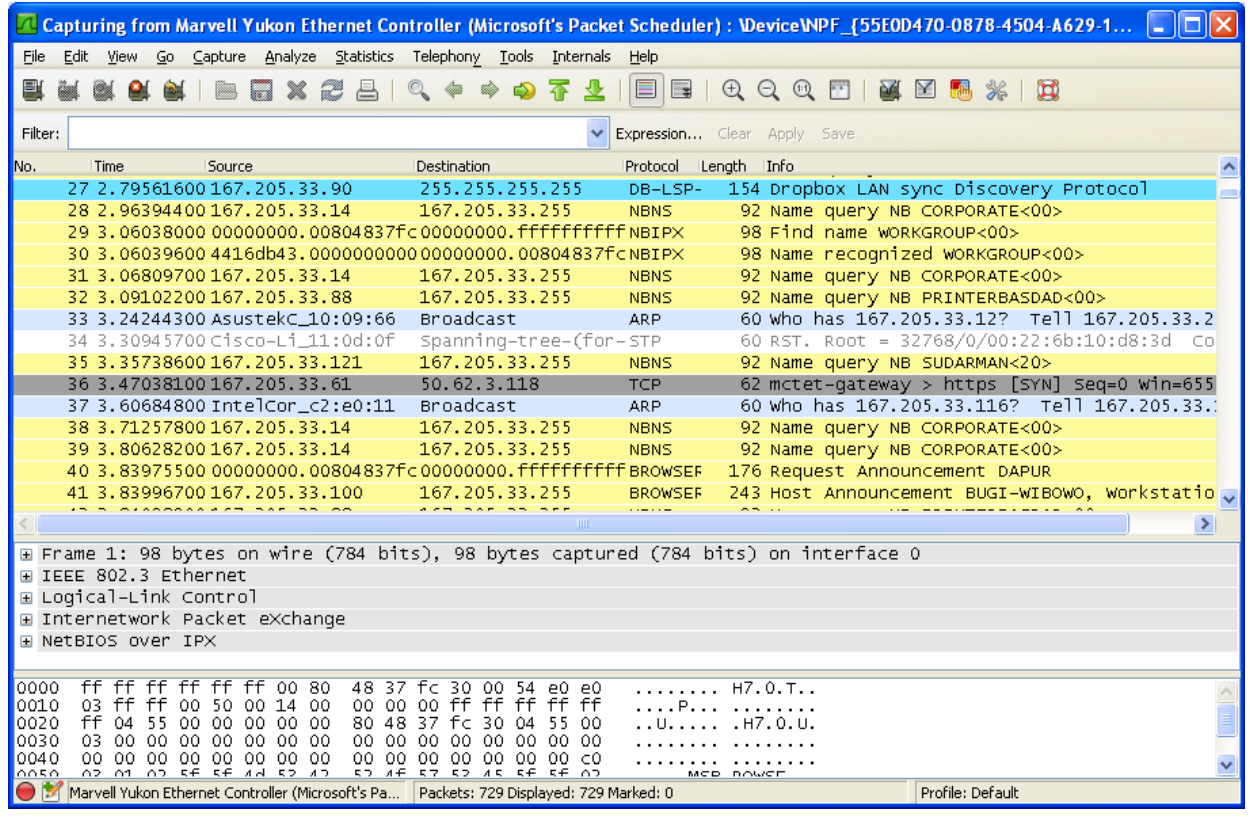
\includegraphics[width=136.71mm,height=227.50mm]{../../images/llm/page_033_img_01.png}%
\end{textblock*}

\end{document}
